\documentclass{beamer}

\usepackage[utf8x]{inputenc}
\usepackage{default}
\usetheme{PaloAlto}
\usecolortheme{seahorse}

\title{Orientação a objetos\\ \textbf{Orientação a objetos em ANSI C - 1}}
\author{Paulo Meirelles, Rodrigo Siqueira}
\date{\today}
\institute{\textbf{Universidade de Brasília - Faculdade do Gama}} 

\begin{document}

%SLIDE INICIAL DE APRESENTAÇÃO
\begin{frame}
  \titlepage
\end{frame}
  
%SLIDES == INTRODUÇÃO
\section{Introdução}
\begin{frame}
  \frametitle{Ferramentas e mais ferramentas...}
  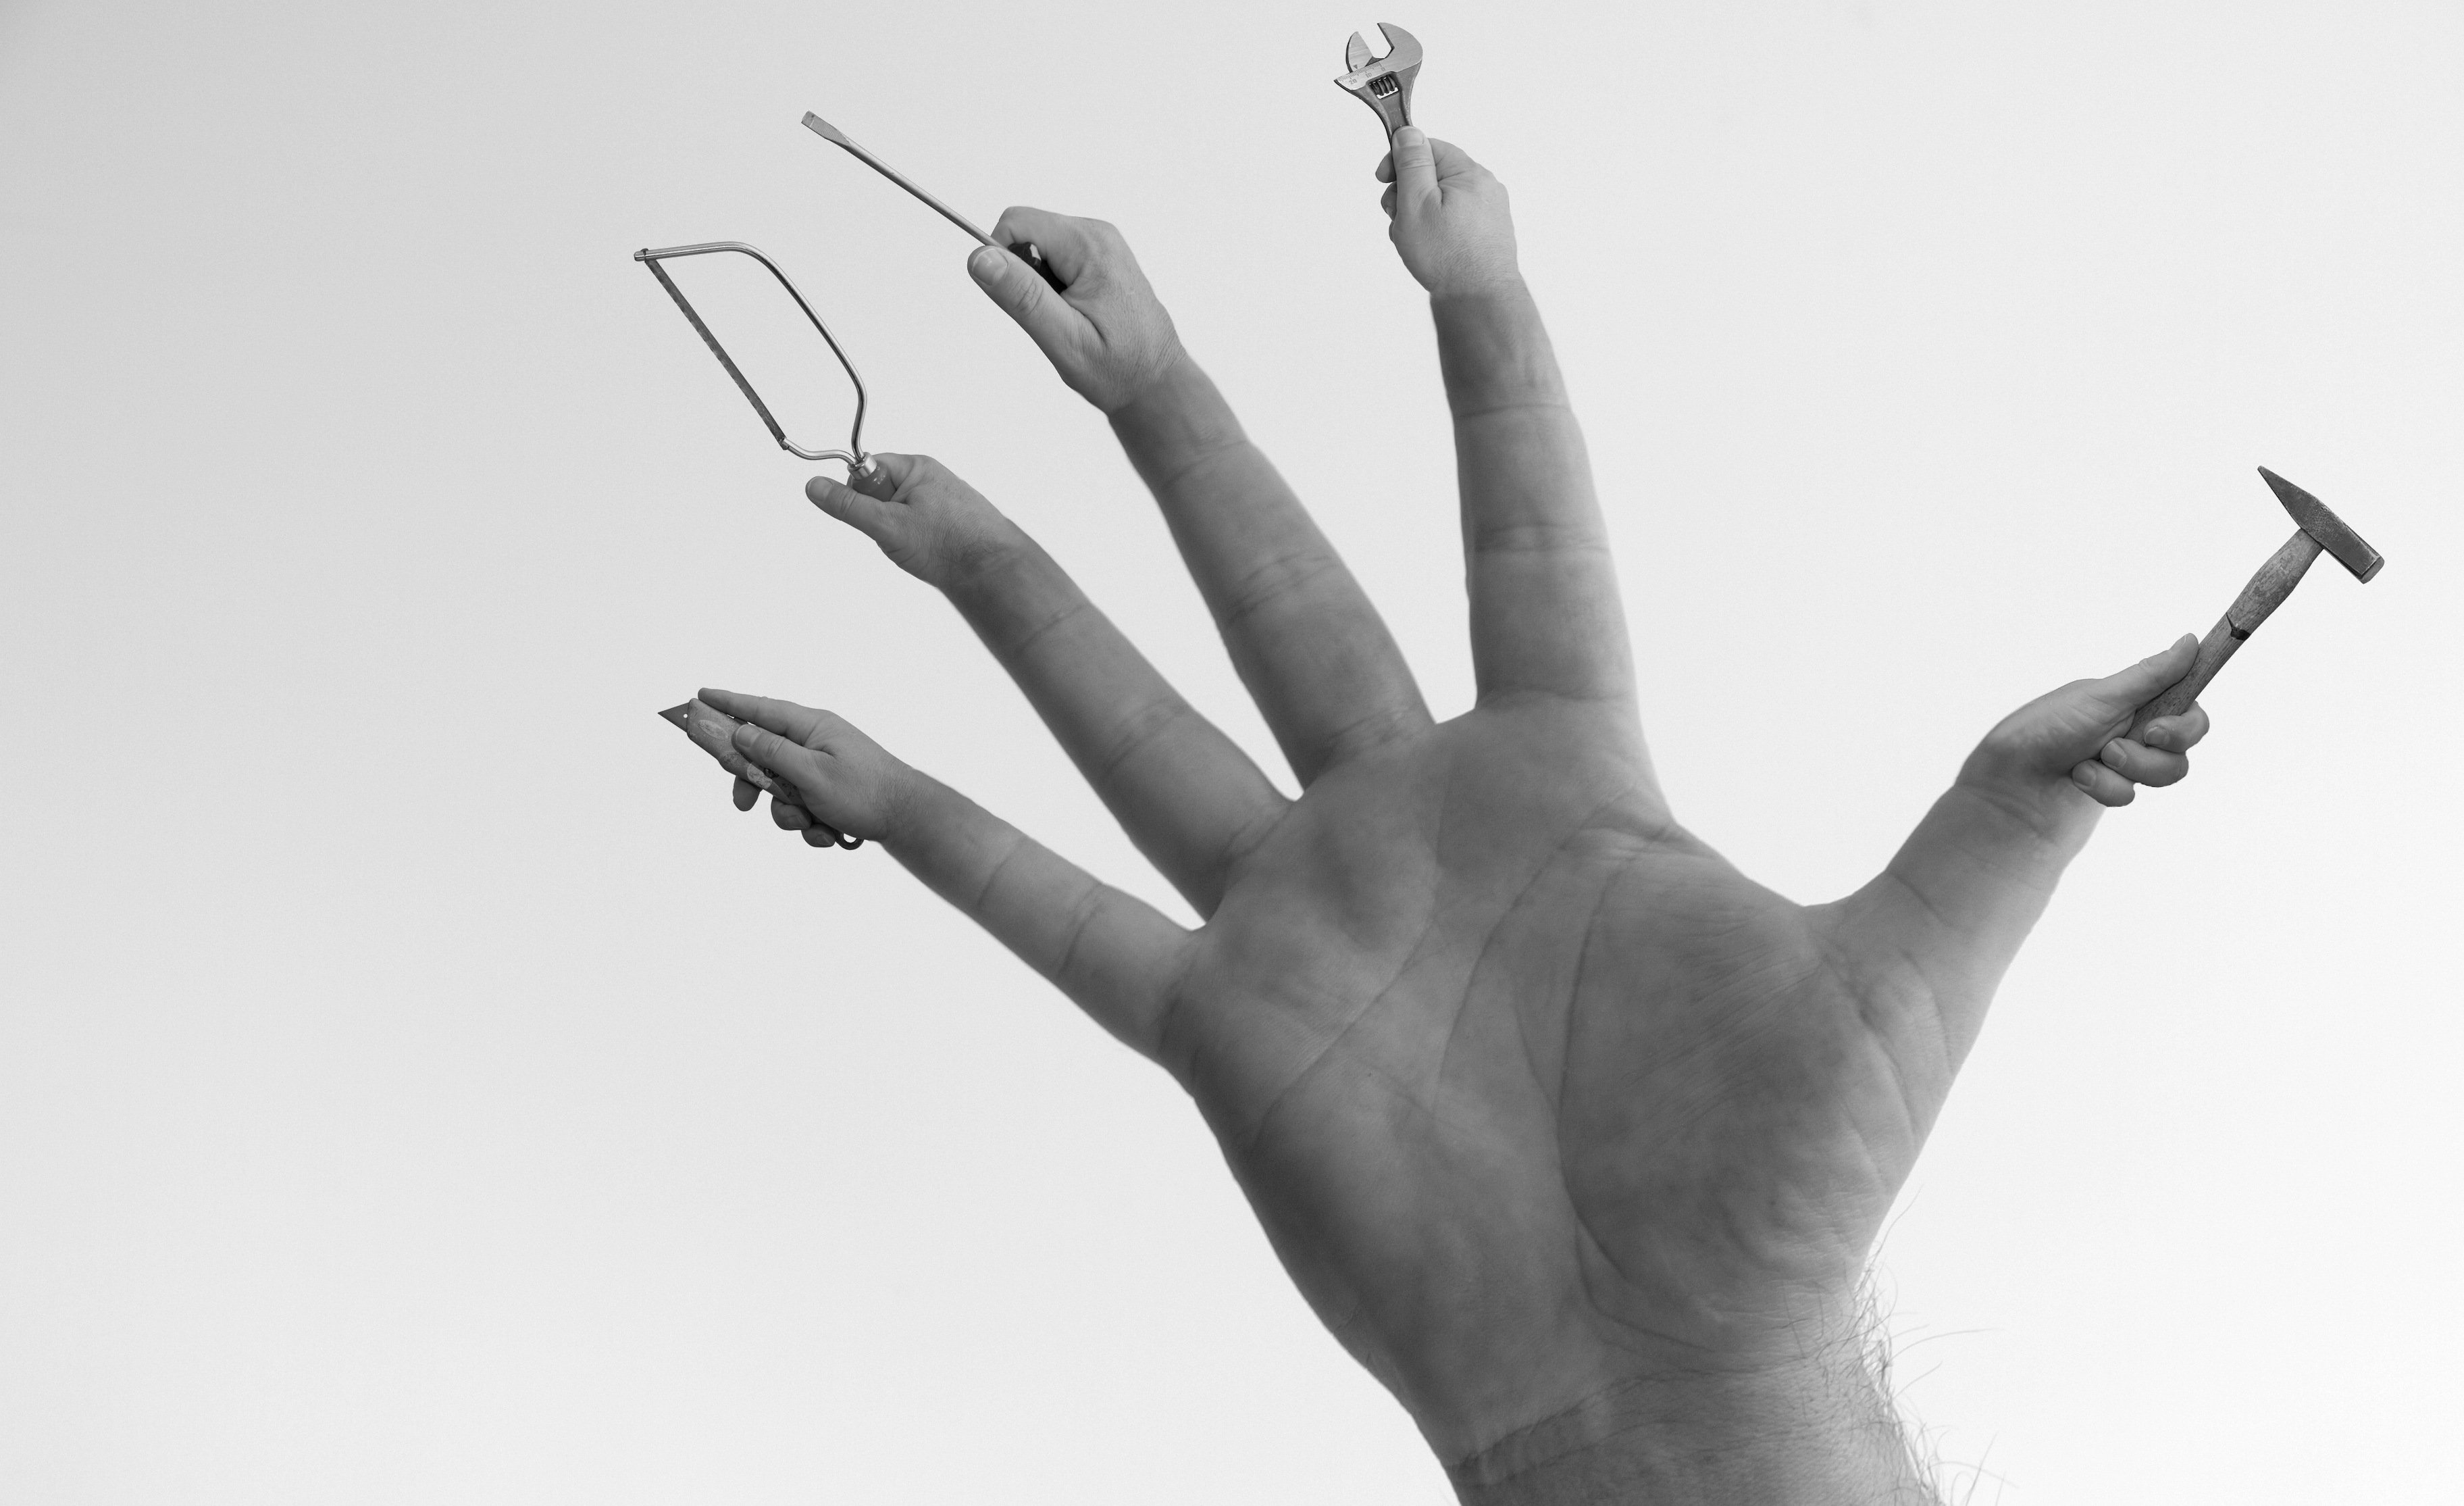
\includegraphics[height = 2in, width = 4in]{image/tools.jpeg}
\end{frame}

\begin{frame}
  \frametitle{Vários caminhos, um único fim}
  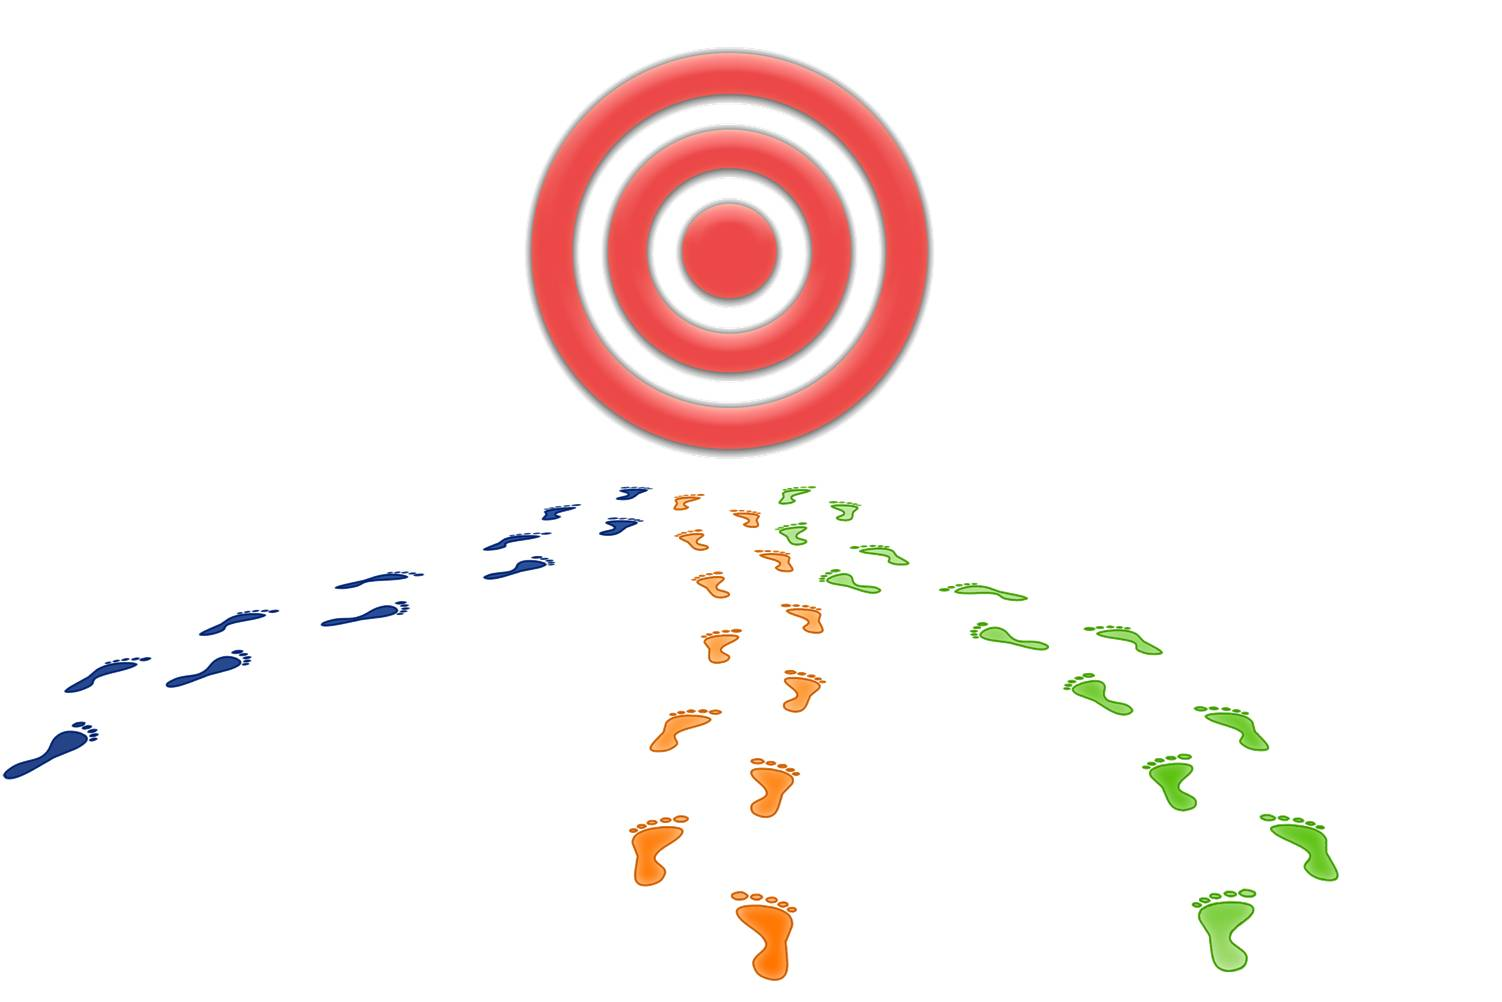
\includegraphics[height = 3in, width = 4in]{image/many_paths.jpg}
\end{frame}

%SLIDES == EXEMPLO
\section{Tipo de dados}

\begin{frame}
  \frametitle{Tipos de dados}
  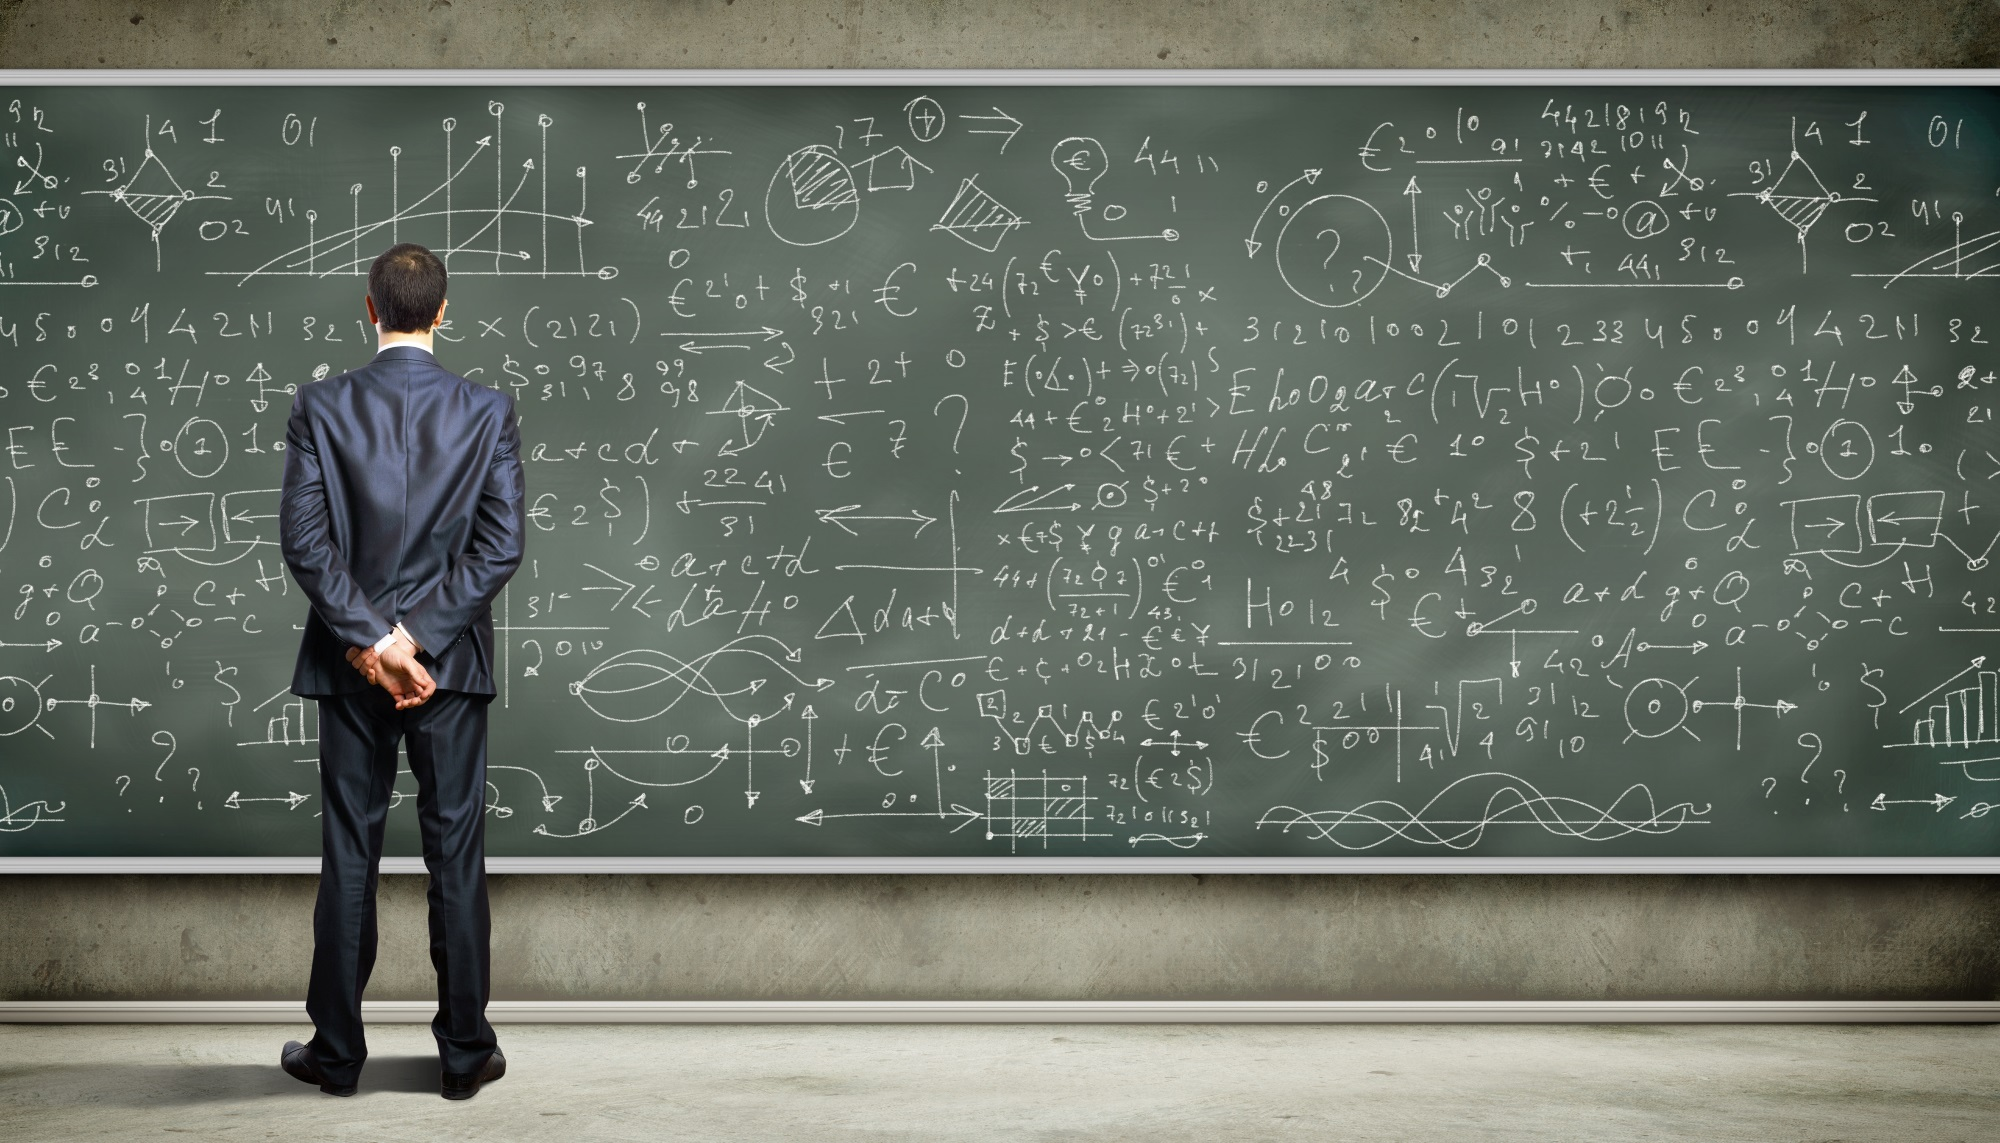
\includegraphics[height = 2in, width = 4in]{image/many_data.jpeg}
\end{frame}

\begin{frame}
  \frametitle{O que são tipos de dados?}
  Pode ser visto como um conjunto de valores.
\end{frame}

\begin{frame}
  \frametitle{O que são tipos de dados?}
  Pode ser visto como um conjunto de valores, mais operações para trabalhar 
  com eles.
\end{frame}

\begin{frame}
 \frametitle{Boas práticas}
 \begin{block}{Primeira boa prática}
  Esconda a representação dos itens de dados e declare apenas os manipuladores 
  necessários.
 \end{block}
\end{frame}

% TIPOS DE DADOS ABSTRATO
\section{Tipo de dados abstrato}

\begin{frame}
  \frametitle{Dados abstratos}
  \includegraphics[height = 3in, width = 4in]{image/abstract.jpeg}
\end{frame}

\begin{frame}
 \frametitle{Dados abstrato}
 \begin{block}{Dados abstrato}
  Chamamos um tipo de dado abstrato, se nos não revelarmos a sua representação 
  para o usuário.
 \end{block}

 \begin{block}{Dividir e conquistar}
  Esconda a informação e divida para conquistar.
 \end{block}
\end{frame}

% Exemplo
\section{Exemplo}
\begin{frame}
  \frametitle{Exemplo}
  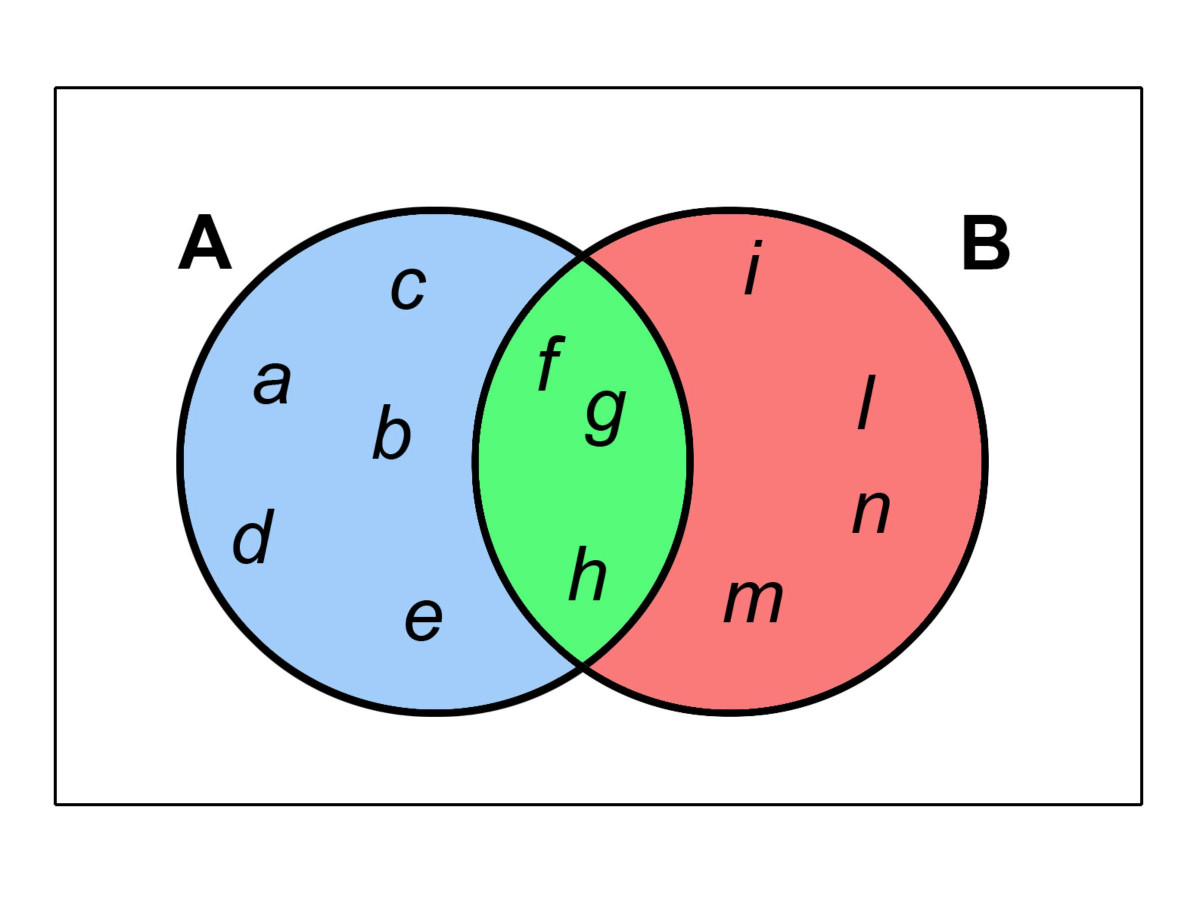
\includegraphics[height = 3in, width = 4in]{image/set.jpg}
\end{frame}

\begin{frame}
  \frametitle{Funções}

  \begin{itemize}
   \item \textbf{add}: Pega algum elemento, adiciona ao conjunto e retorna o 
    ponteiro do o elemento adicionado.
    \begin{itemize}
     \item \textbf{Parâmetros}: conjunto e elemento.
     \item \textbf{Retorna}: ponteiro.
    \end{itemize}
 
   \item \textbf{find}: Procura por um elmento dentro de \textit{set} e retorna 
    o que estiver sido adicionado ou retorna \textit{null}.
    \begin{itemize}
     \item \textbf{Parâmetros}: conjunto e elemento.
     \item \textbf{Retorna}: ponteiro ou \textit{null}.
    \end{itemize}

   \item \textbf{drop}: Localiza um elemento para ser removido do conjunto e 
     retorna o que foi removido.
     \begin{itemize}
      \item \textbf{Parâmetros}: conjunto e elemento.
      \item \textbf{Retorna}: ponteiro.
     \end{itemize}

   \item \textbf{contains}: Converte o resultado de find para \textit{true} ou 
      \textit{False}.
      \begin{itemize}
       \item \textbf{Parâmetros}: conjunto e elemento.
       \item \textbf{Retorna}: inteiro indicando verdadeiro ou falso.
      \end{itemize}

  \end{itemize}
 
\end{frame}

\begin{frame}
  \frametitle{Código}
  Programar...
  \begin{enumerate}
   \item Set.h
  \end{enumerate}

  \begin{center}
    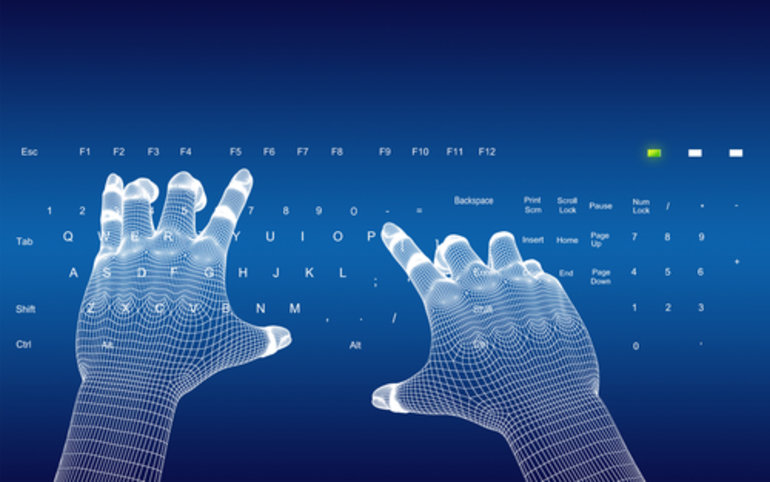
\includegraphics[height = 1.5in, width = 2in]{image/programming.jpg}
  \end{center}
\end{frame}

% GERENCIAMENTO DA MEMÓRIA
\section{Gerenciamento da memória}
\begin{frame}
 \frametitle{Gerenciamento da memória}
 \begin{enumerate}
  \item Como obter um tipo \textit{Set}?
  \begin{itemize}
   \item R: Utilizando ponteiros para referir-se a conjuntos e elementos.
  \end{itemize}
 \end{enumerate}

\end{frame}

\begin{frame}
 \frametitle{Funções}
  \begin{itemize}
   \item \textbf{new}: 
    \begin{itemize}
     \item \textbf{Parâmetros}: Ponteiro para um tipo genérico e ...
     \item \textbf{Retorno}: Uma referência.
    \end{itemize}

   \item \textbf{delete}: Recebe um ponteiro gerado por \textit{new} e recicla 
    o recurso associado.
    \begin{itemize}
     \item \textbf{Parâmetro}: Item para ser removido.
     \item \textbf{Retorno}: Não tem.
    \end{itemize}

  \end{itemize}
\end{frame}

\begin{frame}
  \frametitle{Código}
  Programar...
  \begin{enumerate}
   \item new.h
  \end{enumerate}

  \begin{center}
    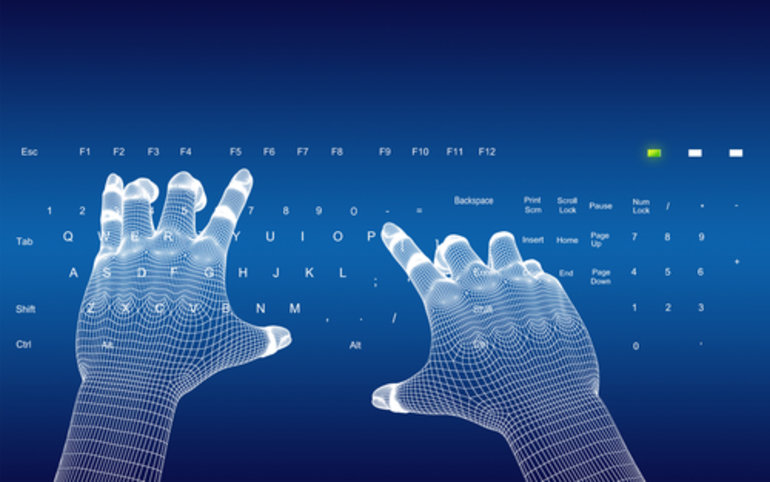
\includegraphics[height = 1.5in, width = 2in]{image/programming.jpg}
  \end{center}
\end{frame}

\begin{frame}
 \frametitle{O que fazer com \textit{Set}?}
 Para que possamos fazer uso de \textit{Set}, é preciso outra abstração de 
  dados conhecida por \textit{Object}.
 \begin{itemize}
  \item \textbf{Object}: Ponteiro para Object.
  \item \textbf{differ}: Compara objetos.
  \begin{itemize}
   \item \textbf{Parâmetros}: duas refêrencias.
   \item \textbf{Retorno}: 
  \end{itemize}

 \end{itemize}
\end{frame}

\begin{frame}
  \frametitle{Código}
  Programar...
  \begin{enumerate}
   \item Object.h
  \end{enumerate}

  \begin{center}
    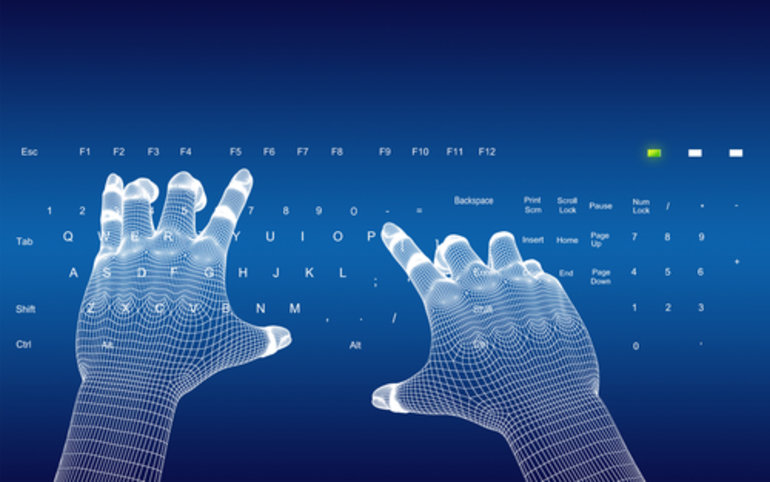
\includegraphics[height = 1.5in, width = 2in]{image/programming.jpg}
  \end{center}
\end{frame}

% EXEMPLO DE UMA APLICAÇÃO
\begin{frame}
  \frametitle{Código}
  Programar...
  \begin{enumerate}
   \item main.c
  \end{enumerate}

  \begin{center}
    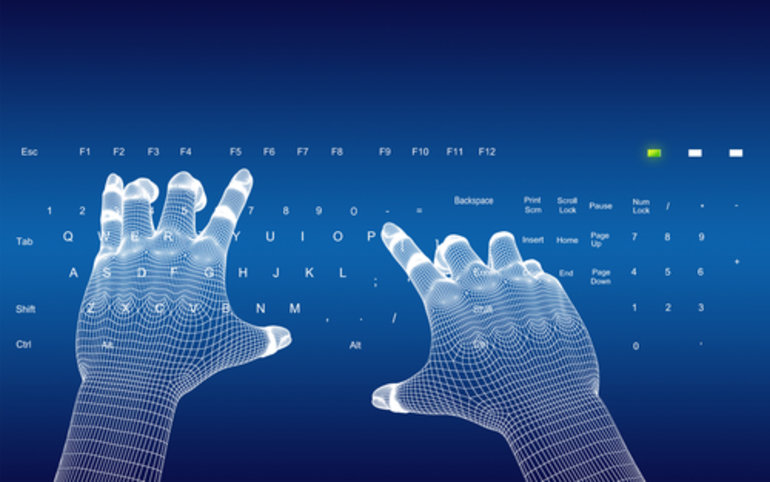
\includegraphics[height = 1.5in, width = 2in]{image/programming.jpg}
  \end{center}
\end{frame}

\section{Implementando uma simplificação de new e delete}
\begin{frame}
 \frametitle{Como funicionará o \textit{new}}
  Se um objeto não armazena informação e se todo objeto pertence a pelo menos 
  um conjunto, podemos representar cada objeto e cada conjunto como um valor 
  inteiro pequeno, único e positivo como índice em um \textit{heap}. \\
  Os objetos apontam para o conjunto que os contém.
\end{frame}

\begin{frame}
 \frametitle{Passo a passo da main e da new}
  \begin{center}
    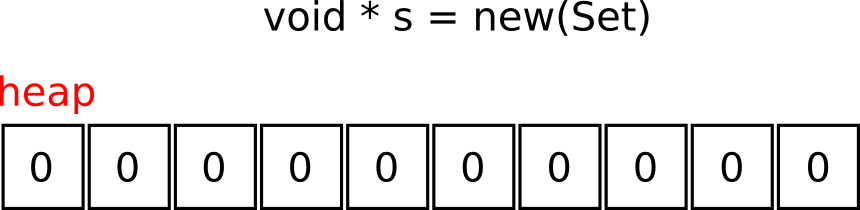
\includegraphics[height = 1in, width = 4in]{image/new_set.png}
  \end{center}
\end{frame}

\begin{frame}
 \frametitle{Passo a passo da main e da new}
  \begin{center}
    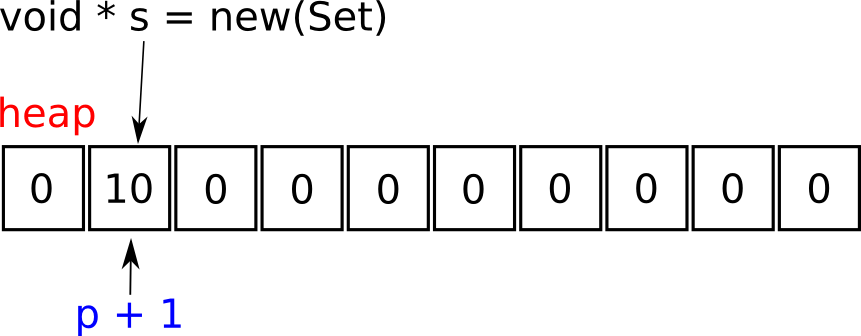
\includegraphics[height = 1.5in, width = 4in]{image/new_set2.png}
  \end{center}
\end{frame}


\begin{frame}
 \frametitle{Passo a passo da main e da new}
  \begin{center}
    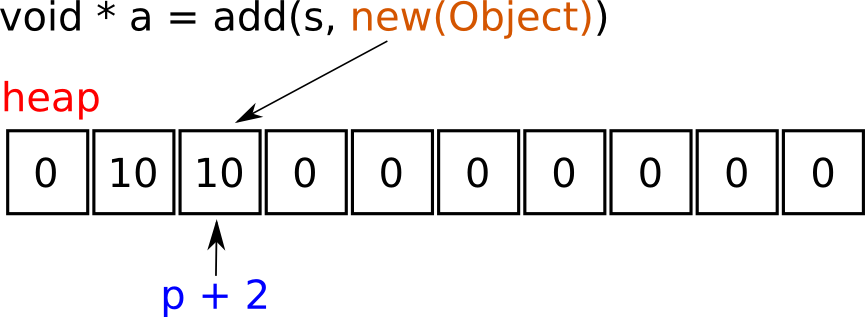
\includegraphics[height = 1.5in, width = 4in]{image/add_a1.png}
  \end{center}
\end{frame}

\begin{frame}
 \frametitle{Passo a passo da main e da new}
  \begin{center}
    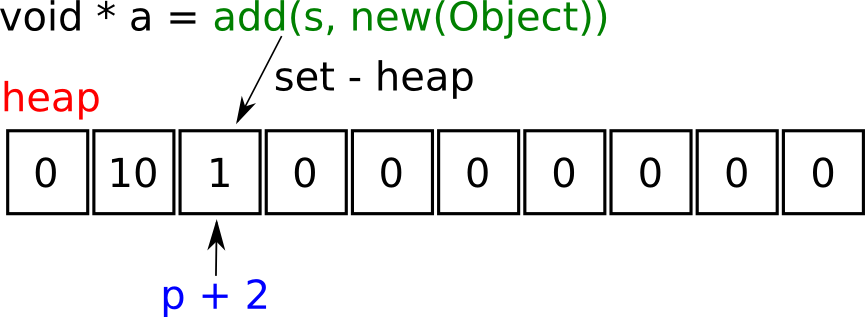
\includegraphics[height = 1.5in, width = 4in]{image/add_a2.png}
  \end{center}
\end{frame}

\begin{frame}
 \frametitle{Passo a passo da main e da new}
  \begin{center}
    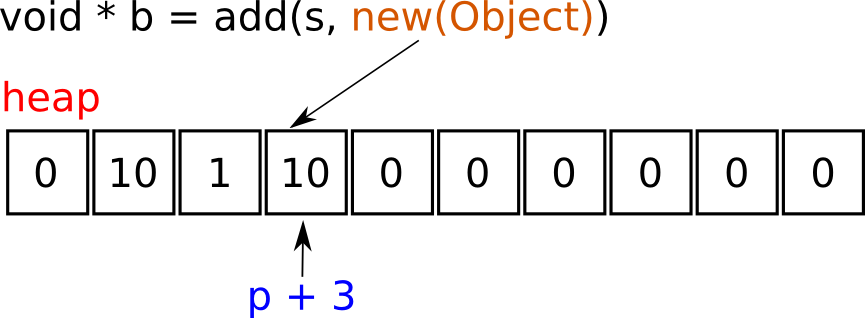
\includegraphics[height = 1.5in, width = 4in]{image/add_b1.png}
  \end{center}
\end{frame}

\begin{frame}
 \frametitle{Passo a passo da main e da new}
  \begin{center}
    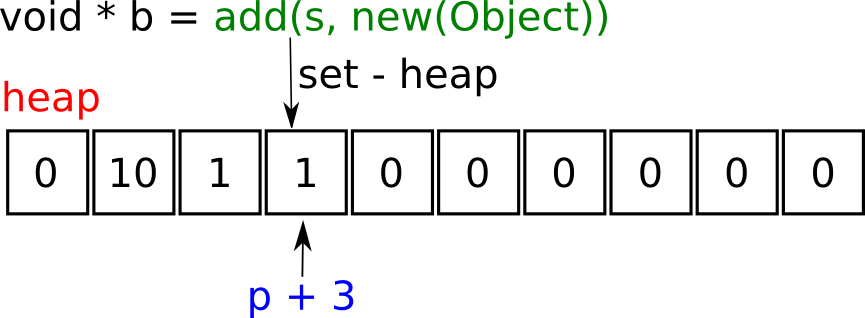
\includegraphics[height = 1.5in, width = 4in]{image/add_b2.png}
  \end{center}
\end{frame}

\begin{frame}
 \frametitle{Passo a passo da main e da new}
  \begin{center}
    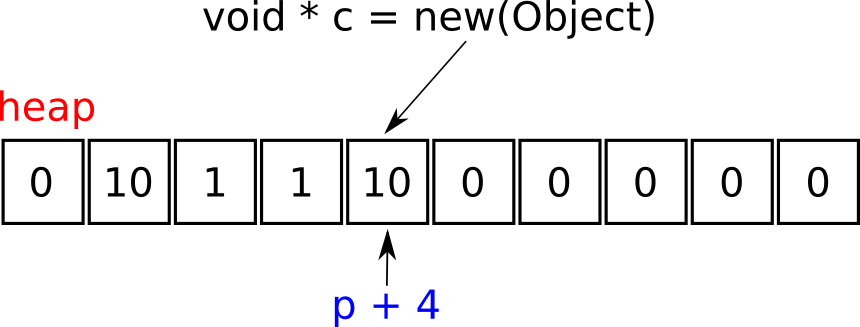
\includegraphics[height = 1.5in, width = 4in]{image/new_c.png}
  \end{center}
\end{frame}

\begin{frame}
  \frametitle{Código}
  Programar...
  \begin{enumerate}
   \item new.c, set.c e object.c
  \end{enumerate}

  \begin{center}
    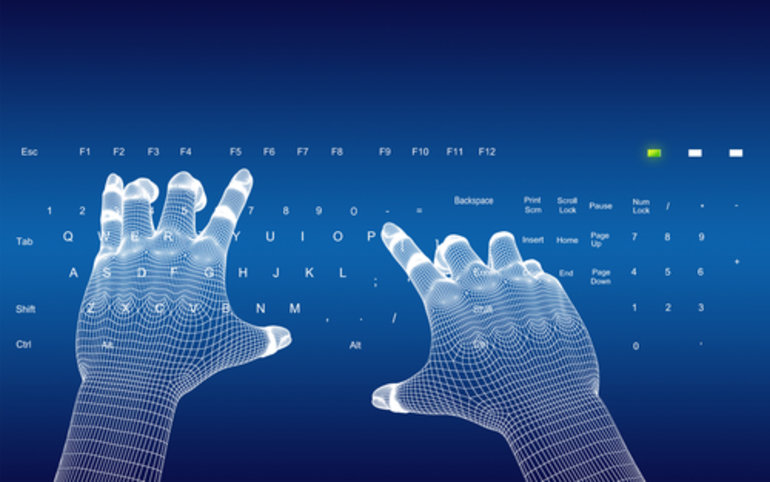
\includegraphics[height = 1.5in, width = 2in]{image/programming.jpg}
  \end{center}
\end{frame}

% SOFISTICANDO A SOLUÇÃO
\section{Melhorando a solução (bag)}

\begin{frame}
 \frametitle{Level up - Second round}
 \begin{center}
    
\includegraphics[height = 2in, width = 3in]{image/levelup.jpg}
  \end{center}
\end{frame}

\begin{frame}
 \frametitle{Bag}
  A utilização de array não é apropriada, uma solução melhor consiste em criar 
  um conjunto onde cada elemento tem uma referência ao conjunto e um contador.

  \begin{enumerate}
   \item Representar \textit{Set} como uma \textit{struct} que armazena a 
     quantidade de elementos adicionados.
   \item Fazer com que \textit{Object} saiba quando foi inserido e mantenha uma 
    refência ao conjunto que pertence.
  \end{enumerate}

\end{frame}

\begin{frame}
  \frametitle{Código}
  Programar...
  \begin{enumerate}
   \item Reimplementar: new, add, find e drop
  \end{enumerate}

  \begin{center}
    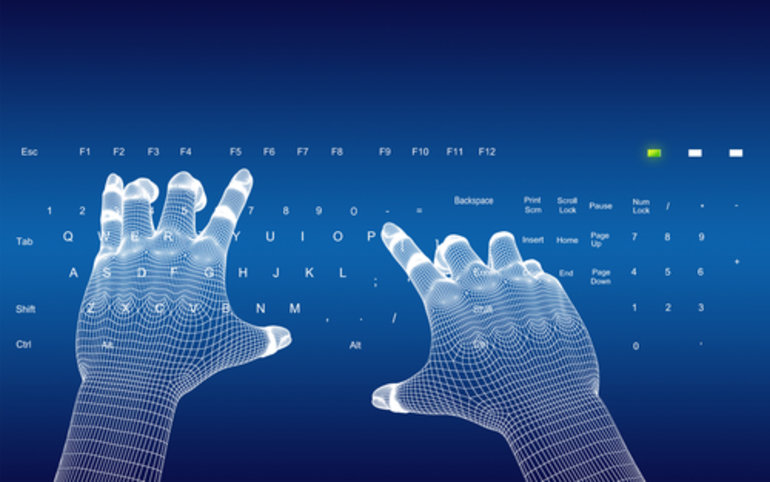
\includegraphics[height = 1.5in, width = 2in]{image/programming.jpg}
  \end{center}
\end{frame}

\begin{frame}
 \frametitle{Final}
 
 \begin{center}
    
\includegraphics[height = 2in, width = 2in]{image/levelup2.jpg}
  \end{center}

\end{frame}

\end{document}
